\documentclass[tikz, border = 2mm]{standalone}
% \usepackage{kompendium-figurer}
\usepackage{pgfplots}
\usepgfplotslibrary{fillbetween}

    \pgfkeys{/pgfplots/Delta Style/.style={
		    % scale only axis,
		    grid=major,
		    % axis equal,
		    grid style={dashed, gray!30}, %Uncomment these lines for no grid
		    axis lines=middle,
		    inner axis line style={=stealth}, %Arrow type
        ultra thick,
		    xlabel={\large $x$},
		    ylabel={\large $z$},
        cycle list = {black,black!70,black!40,black!10} %Plot colors cycle in grayscale
      }}

    \pgfplotsset{
        % use this `compat' level or higher to use the LUA backend for calculation
        % (--> speed improvement)
        compat=1.12,
        % declare your function here ...
        /pgf/declare function={
            f(\x) = 4*x^2;
        },
        /pgf/declare function={
            T(\x) = 4;
        },
    }

\begin{document}
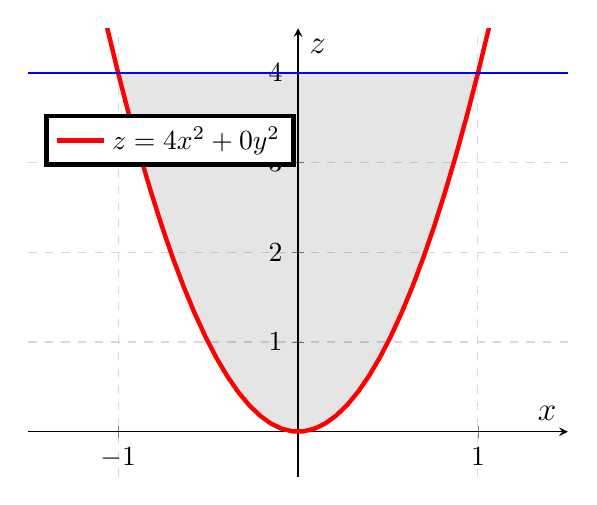
\begin{tikzpicture}
  \begin{axis}[
    Delta Style,
    legend pos =north west,
    legend cell align={left},
    legend style={at={(0.03,0.75)},anchor=west},
    ytick={1,2,...,18},
    xtick={-1,0,...,1},
    ymin=-0.5,
    ymax=4.5,
    xmin=-1.5,
    xmax=1.5,
		]
    % Filling
    \addplot[name path=plot,ultra thick,red,samples=100,domain= -3:3] {f(x)};
    \addlegendentry{$z = 4x^ 2 + 0y^2$};
    \addplot[name path=line,thick,blue,samples=100,domain= -3:3] {T(x)};
    
    \addplot [
        thick,
        color=black,
        fill=black,
        fill opacity=0.1
    ]
    fill between[
        of=plot and line,
        soft clip={domain=-1:1},
    ];

    
    % \addlegendentry{$z = 4 - 11x + 9x^2 + 2^2 + x\cdot 2$};
    \addplot[color=gray,fill=white,only marks,mark size = 4pt] coordinates {(1,8)};
		\end{axis}
	\end{tikzpicture}
\end{document}